\section{Tool Demonstration}
\label{sec:demo}

Discuss the main steps of process that needs to be followed for synthezing
and performing the conformance analysis,that are, 

\subsection{Glossary building and terms definition}
The first step towards writing the controller specifications as a natural
language in EARS-CTRL is to define the glossary terms. 
The user is provided with a projectional editor
(figure~\ref{fig:glossary_def}) to define glossary terms for the following,
1) components that interface with the controller, 2) sensors and actuators those components make available to the controller and 3) rules between
signals definitions.
\begin{figure*}[!h]
\centering
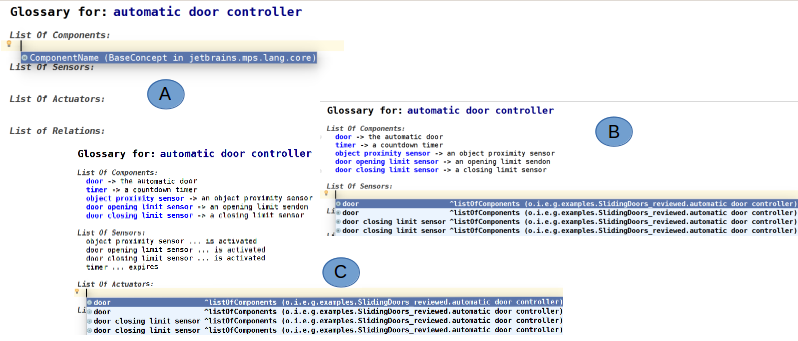
\includegraphics[width=1\textwidth]{./images/glossary_def1.png}
\caption{step-by-step glossary building for sliding door controller: (A)
Components definition, (B) Sensors definition and (C) Actuators definition}
\label{fig:glossary_def}
\end{figure*}

\subsection{EARs-based requirements building for the controller}

\begin{figure*}[!h]
\centering
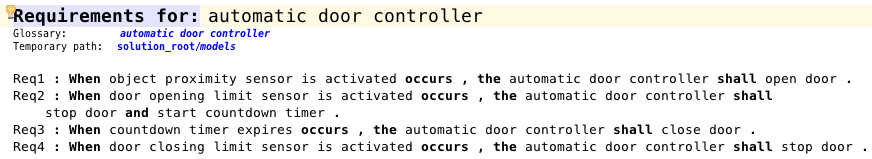
\includegraphics[width=1\textwidth]{./images/EARS-Reqs.png}
\caption{EARS requirements for sliding door}
\label{fig:EARS_req}
\end{figure*}

\subsection{Synthesizing the EARs-based requirements}
\subsection{Simulation and Test Cases}
\subsubsection{interfacing with Simulink}
\subsubsection{setting up test case parameters}
\subsubsection{obtaining results and conformance analysis}